\chapter{Métodos Empíricos em Engenharia de Software}

\section{Métodos Ágeis}
Os negócios atualmente operam em um ambiente global sujeito a rápidas mudanças sendo crucial estar preparado para novas oportunidades de mercado, mudanças de condições econômicas e ao surgimento de produtos e serviços concorrentes. O software é um dos componentes cruciais para a realização de várias operações de negócio e realizá-lo de forma rápida também é uma maneira de aproveitar novas oportunidades e responder às pressões competitivas \cite{sommerville_2006}.

O manifesto ágil \cite{beck2001agile} consiste na base que fundamenta o desenvolvimento ágil de
software sendo composto de quatro valores fundamentais:

\begin{itemize}
    \item \textbf{Os indivíduos e suas interações} acima de procedimentos e ferramentas;
    \item \textbf{O funcionamento do software} acima de documentação abrangente;
    \item \textbf{A colaboração dos clientes} acima da negociação de contratos;
    \item \textbf{A capacidade de resposta a mudanças} acima de um plano pré-estabelecido.
\end{itemize}

\textit{``Enquanto há valor nos itens à direita, valorizamos mais os itens à esquerda''} \cite{beck2001agile}.

Além desses valores são definidos 12 princípios de agilidade:

\begin{itemize}
    \item Nossa maior prioridade é satisfazer o cliente, através da entrega adiantada e contínua de software de valor;
    \item Aceitar mudanças de requisitos, mesmo no fim do desenvolvimento. Processos ágeis se adequam a mudanças, para que o cliente possa tirar vantagens competitivas;
    \item Entregar software funcionando com freqüencia, na escala de semanas até meses, com preferência aos períodos mais curtos;
    \item Pessoas relacionadas a negócios e desenvolvedores devem trabalhar em conjunto e diariamente, durante todo o curso do projeto;
    \item Construir projetos ao redor de indivíduos motivados. Dando a eles o ambiente e suporte necessário, e confiar que farão seu trabalho;
    \item O Método mais eficiente e eficaz de transmitir informações para, e por dentro de um time de desenvolvimento, é através de uma conversa cara a cara;
    \item Software funcional é a medida primária de progresso;
    \item Processos ágeis promovem um ambiente sustentável. Os patrocinadores, desenvolvedores e usuários, devem ser capazes de manter indefinidamente, passos constantes;
    \item Contínua atenção à excelência técnica e bom design, aumenta a agilidade;
    \item Simplicidade: a arte de maximizar a quantidade de trabalho que não precisou ser feito;
    \item As melhores arquiteturas, requisitos e designs emergem de times auto-organizáveis;
    \item Em intervalos regulares, o time reflete em como ficar mais efetivo, então, se ajustam e otimizam seu comportamento de acordo.
\end{itemize}

Nem todos os processos ágeis aplicam tais princípios de maneira igualitária e alguns modelos escolhem ignorar (ou ao menos minimizar) a importância de um ou mais princípios \cite{pressman_2009}.

Processos de desenvolvimento ágeis geralmente são iterativos onde a
especificação, projeto, desenvolvimento e teste são intercalados. O software é desenvolvido
em uma série de incrementos e cada incremento fornece uma nova funcionalidade ao sistema \cite{sommerville_2006}. As duas principais
vantagens de se adotar uma abordagem incremental para o desenvolvimento de software são:

\begin{itemize}
    \item Entrega acelerada dos serviços ao cliente. Os clientes poderão obter valor do sistema já nos incrementos iniciais;
    \item Engajamento do usuário com o sistema. Os usuários do sistema devem estar envolvidos no processo
    de desenvolvimento dando \textit{feedback} à equipe de desenvolvimento sobre os incrementos entregues.
\end{itemize}

    \subsection{\textit{Extreme Programming}}
    \textit{Extreme Programming} (XP) é uma filosofia de desenvolvimento de software baseada nos valores de comunicação, simplicidade, \textit{feedback} e coragem. É designado para se trabalhar com projetos que podem ser
    construídos por equipes de dois a dez programadores, os quais não devem possuir limitações
    por causa do ambiente computacional e possam ser capazes de realizar testes de
    software em uma fração de um dia \cite{beck_2004}.

    No XP, são definidas 12 importantes práticas que auxiliam no
    desenvolvimento de software e em suas \textit{releases}.
    Uma \textit{release} consiste no lançamento, parcial ou não,
    de um software, sendo que em muitas das vezes são
    lançadas versões beta do mesmo, proporcionando, assim, uma possível
    fase de \textit{debugging} ou \textit{feedback}, provinda do
    cliente ou até mesmo da equipe de desenvolvimento. As práticas do XP, por sua vez, alinham-se bem no decorrer do ciclo de desenvolvimento de software e são includentes, ou seja, onde uma possui determinada desvantagem, outra
    irá compensar com seus pontos positivos \cite{beck_2004}. As práticas são:

    \begin{itemize}
        \item Cliente Presente: clientes devem sempre estar presentes para auxiliarem a equipe com seus \textit{feedbacks}.
        \item \textit{Design} Simples: o sistema deve sempre ser desenhado de forma o mais simples possível, sendo que complexidades encontradas devem ser removidas rapidamente.
        \item Integração Contínua: integração e construção do sistema muitas vezes ao dia, sempre que uma tarefa
        for concluída.
        \item Jogo do Planejamento (do inglês \textit{Planning Game}): determina de maneira rápida o escopo de uma \textit{release} combinando prioridades de negócio e estimativas técnicas.
        \item Metáfora (do inglês \textit{Metaphor}): linguagem comum que os membros devem possuir para poderem explicar facilmente como o sistema funciona como um todo.
        \item Padrões de Codificação: escrita do código de acordo com boas práticas de programação, enfatizando uma comunicação através do mesmo.
        \item Programação em Pares: realizar a codificação do sistema sempre
        com dois programadores que compartilham a mesma máquina.
        \item Propriedade Coletiva: qualquer pessoa pode modificar, desde que esteja realizando de maneira correta, qualquer parte do código a qualquer momento.
        \item Refatoração: reestruturação do sistema sem alteração de seu comportamento, objetivando
        remover duplicidade, simplificação de código, aumento de flexibilidade e melhoramento da comunicação.
        \item Semana de 40 horas: o trabalho semanal realizado não pode ultrapassar o limite de 40 horas.
        \item Teste: são escritos testes unitários, que devem funcionar de maneira adequada para que
        o desenvolvimento do sistema continue.
        \item Versões Pequenas: colocar rapidamente um sistema simples e funcional em produção, para que posteriormente sejam lançadas novas versões do mesmo em um curto período de tempo.
    \end{itemize}

    \subsection{Kanban}
    O Kanban \cite{radigan_2015} é um \textit{framework} que visa auxiliar equipes a organizarem de maneira mais prática suas tarefas. Utiliza um quadro de produção, figura \ref{kanban}, que irá conter todo o fluxo de trabalho, possuindo três principais colunas:

    \begin{itemize}
        \item \textit{To Do}: tarefas que serão realizadas em breve.
        \item \textit{In Proguress}: tarefas que atualmente estão sendo realizadas pela equipe.
        \item \textit{Done}: tarefas que foram finalizadas.
    \end{itemize}

    \begin{figure}[!htpb]
        \centering
        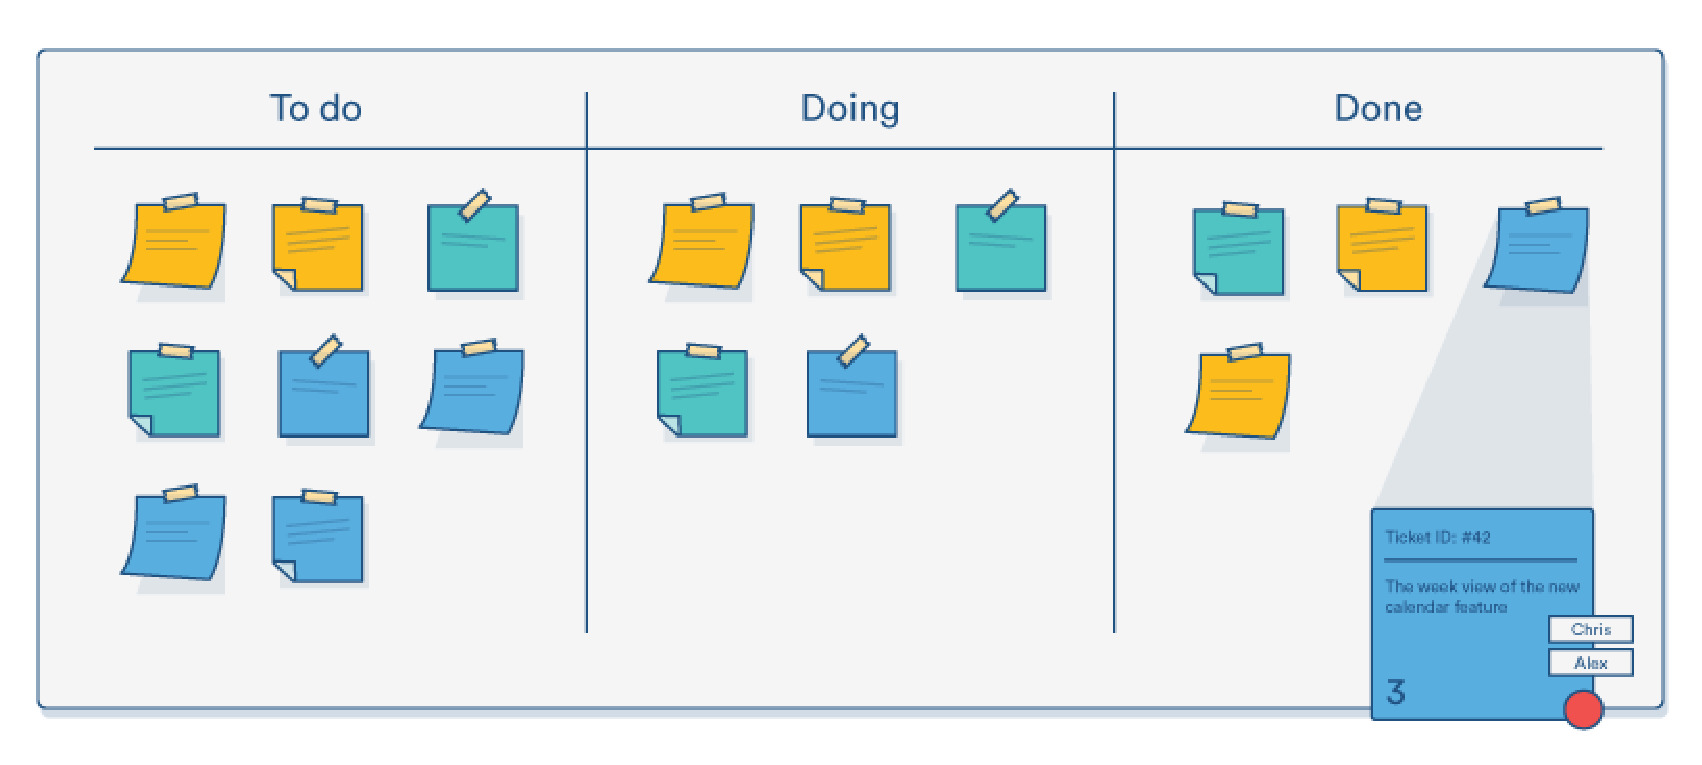
\includegraphics[keepaspectratio=true,scale=0.5]{figuras/kanban.eps}
        \caption{Quadro Kanban de produção. Fonte: \cite{radigan_2015}}
        \label{kanban}
    \end{figure}

    Cada vez que uma tarefa passar por mudanças que alterem seu estado, o quadro deve ser atualizado, trazendo mais transparência para a equipe. Além disso, tarefas que são planejadas e não se encaixam no contexto vigente do quadro são armazenadas no \textit{Backlog}.

\section{Requisitos de Software}
Entender os requisitos de um problema é uma das difíceis missões
que são encaradas na Engenharia de Software. Em muitos casos, o cliente não sabe o que realmente quer ou até mesmo
suas acaba mudando suas necessidades com o decorrer do projeto.   Sommerville \cite{sommerville_2006} define os requisitos de um projeto como ``requisitos do usuário'' e ``requisitos do sistema''. Os requisitos de usuários consistem de declarações, em
linguagem natural, que o sistema deve fornecer e restrições que o mesmo deve
operar. Os requisitos de sistema estabelecem de maneira detalhada as
funções e restrições do sistema. Além disso, os requisitos de sistema
classificam-se em funcionais e não funcionais:

\begin{itemize}
    \item Requisitos Funcionais: declaração de funções que o sistema deve fornecer, como o mesmo irá reagir com certas entradas e como deve se comportar para certas situaçoes.
    \item Requisitos não Funcionais: restrições sobre serviços ou funções oferecidas pelo sistema.
\end{itemize}

O levantamento adequado de requisitos de software é crucial para que possa ser feito um mapeamento das reais necessidades do cliente com funcionalidades que um sistema deve atender. Thayer \cite{thayer_1997} define a Engenharia de Requisitos como um processo que provê os mecanismos apropriados para o entendimento do que o cliente quer, analisando a necessidade, avaliando a viabilidade, negociando uma solução inteligente, especificando a solução de maneira não ambígua, validando a especificação e gerenciando os requisitos conforme os mesmos são transformados em um sistema operacional.

Dentre as atividades da Engenharia de Requisitos encontra-se a elicitação de requisitos, a qual, para Leite \cite{leite_1994}, é reponsável por identificar todos os fatos que irão fazer parte dos requisitos do sistema, buscando fornecer todo o entendimento que o software deve possuir.

Com os requisito do sistema em mãos é possível identificar os seus casos de usos, que são de narrativas ou modelos de texto que descrevem uma função ou recurso do sistema do ponto de vista do usuário \cite{pressman_2009}. Em um contexto ágil, como por exemplo o XP, o propósito do caso de uso é mapeado na estória de usuário. Estórias de usuário são escritas pelos clientes como coisas que o sistema precisa fazer por eles, servem para propor estimativas para uma \textit{release} e seus tempos de realização devem ser curtos, entre uma a três semanas de desenvolvimento \cite{beck_2004}.

\section{Teste de Software}
Teste de software é o processo de execução de um produto para averiguar se ele atingiu suas especificações e funciona corretamente em seu ambiente alvo \cite{artigo_intro_teste}.

De acordo com \citeonline{sw_test_tech}, um bom teste é o que possui uma alta probabilidade de encontrar um erro ainda não descoberto e um teste bem sucedido é o que de fato descobre erros desconhecidos.

Esses testes são estruturados em níveis, cada um com um determinado objetivo dentro do conjunto de testes, de modo a garantir a qualidade do produto em desenvolvimento \cite{sw_test_tech}.

    \subsubsection{Testes Unitários}
    Testes unitários possuem como objetivo verificar a existência de defeitos em cada módulo do projeto. Seu alvo são os métodos desenvolvidos ou pequenos trechos específicos de código \cite{artigo_intro_teste}.

    É realizado durante o desenvolvimento, pelo próprio desenvolvedor, pois testa a unidade básica de software, que é o menor ``pedaço''  testável, por sua vez chamado de unidade, dando origem ao nome deste tipo de teste \cite{sw_test_tech}.

    Um exemplo de objetivo do teste unitário é a procura pela identificação de erros de lógica e de implementação \cite{maldonado}.

\section{Gerência de Configuração de Software}
Um sistema pode ser definido como a combinação de elementos que entre si interagem e estão organizados para alcançar um ou mais objetivos previamente declarados, onde suas características físicas e funcionais de \textit{hardware} ou software representam sua configuração \cite{SWEBOK2014}.

Em uma definição mais formal, a ISO 24765 \cite{iso_24765} define Gerência de Configuração como uma disciplina responsável por: ``identificar e documentar as características funcionais e físicas de um item de configuração, controlar as alterações dessas características, registar e reportar o processamento de alterações e o \textit{status} de implementação, e verificar a conformidade com os requisitos especificados''.

A Gerência de Configuração de Software (SCM, do inglês \textit{Software Configuration Management}) é um processo que beneficia o gerenciamento de projeto, assim como o seu desenvolvimento, manutenção e atividades referentes à garantia de qualidade \cite{SWEBOK2014}.

O CMMI-DEV \cite{cmmi_dev} define 3 objetivos para a Gerência de Configuração de Software:
\begin{itemize}
    \item Estabelecimento de \textit{Baselines}: para cada nova mudança implementada um incremento na evolução do projeto é gerado. Essas mudanças devem possuir um histórico bem definido. As ferramentas de controle de versão facilitam esse trabalho, além de possibilitarem uma programação concorrente.
    \item Rastreamento e Controle de Mudanças: durante o desenvolvimento de software mudanças ocorrem com frequência. É necessário portanto que as mesmas sejam armazenadas, analisadas e agrupadas de acordo com o histórico e suas prioridades.
    \item Estabelecimento de Integridade: verificar se a construção de um sistema, atendendo suas configurações pré-estabelecidas, é bem sucedida a cada nova mudança registrada.
\end{itemize}

\section{Software Livre}
``O Software livre é aquele que permite aos usuários usá-lo, estudá-lo, modificá-lo e redistribui-lo, em geral, sem restrições para tal e prevenindo que não sejam impostas restrições aos futuros usuários'' \cite{meirelles2013}.

Em comparação ao software restrito, o software livre apresenta algumas vantagens devido ao fato de seu código-fonte estar disponível para qualquer usuário, partindo do princípio que seu licenciamento esteja de acordo com as definições da \textit{Free Software Foundation}\footnote{\url{http://www.gnu.org/philosophy/free-sw.pt-br.html}} ou da \textit{Open Source Initiative}\footnote{\url{https://opensource.org/docs/definition.html}}. Essa disponibilidade auxilia no desenvolvimento de aplicações personalizadas, uma vez que que é possível partir de uma solução já existente ao invés de desenvolver tudo partindo do zero. Tal abordagem possui um impacto significativo na redução de custos e diminuição na duplicação de esforço \cite{meirelles2013}.

Raymond \cite{raymond1999}, observando o modelo de desenvolvimento do Linux, percebeu que o compartilhamento de código possivelmente melhoraria a qualidade final de uma aplicação, uma vez que uma quantidade grande de desenvolvedores, com diferentes habilidades e conhecimentos, conseguem propor melhorias e consertar \textit{bugs} em uma pequena quantidade de tempo \cite{meirelles2013}.

\section{Usabilidade de Software}
A usabilidade é geralmente considerada como o fator que assegura que
os produtos sejam fáceis de usar, eficientes e agradáveis, sob a
perspectiva do usuário, através da otimização das interações
estabelecidas pelas pessoas com produtos interativos \cite{rogers_2013}.

Segundo a ISO 9126 \cite{iso9126}, o conceito de usabilidade, em um contexto de software, é definido como "capacidade do produto de software de ser entendido, aprendido, usado e atraente para o usuário, quando usado em condições especificadas". Nielsen \cite{nielsen_1994} propõe que a usabilidade está distribuida em diversos elementos e define alguns fatores que estão associados a mesma, sendo esses:

\begin{itemize}
    \item Eficiência: proporcionar ao usuário o cumprimento do seu objetivo de forma rápida e fácil. Para isso, uma aplicação deve ser feita de forma simples, com o mínimo de poluição visual possível, intuitiva e bem estruturada, reduzindo o esforço e a dificuldade em se realizar um determinada tarefa.
    \item Facilidade de Aprendizagem: capacidade do cliente aprender rapidamente utilizar o sistema de maneira intuitiva.
    \item Facilidade de Memorização: o sistema deve ser capaz de ser facilmente memorizado, ou seja, por mais que um usuário fique um tempo sem utilizá-lo, o mesmo irá se recordar facilmente de como se usa.
    \item Satisfação: a utilização do sistema deve providenciar ao usuário uma experiência agradável.
    \item Seguraça: refere-se a prevenção para que o usuário não cometa erros. Uma aplicação deve conter botões de desfazer, botões de edição, pedidos de confirmação de ação antes da mesma ser realizada e dicas de como proceder em determinadas situações.
\end{itemize}

\section{Qualidade de Software}

\subsection{Métricas de Software}
% Developing or selecting high quality software products is therefore of prime importance. Comprehensive specification and evaluation of software product quality is a key factor in ensuring adequate quality. This can be achieved by defining appropriate quality characteristics, taking account of the purpose of usage of the software product. It is important that every relevant software product quality characteristic is specified and evaluated, whenever possible using validated or widely accepted metrics.

% As quality characteristics and associated metrics can be useful not only for evaluating a software product but also for defining quality requirements and other usage, ISO/IEC 9126 (1991) has been replaced by two related multipart standards: ISO/IEC 9126 (Software product quality) and ISO/IEC 14598 (Software product evaluation). The software product quality characteristics defined in this part of ISO/IEC 9126 can be used to specify both functional and non-functional customer and user requirements.
